\documentclass[11pt,a4paper]{article}

\usepackage[margin=2.2cm]{geometry}
\usepackage{graphicx}
\usepackage{booktabs}
\usepackage{amsmath}
\usepackage{xcolor}
\usepackage{caption}
\usepackage{float}
\usepackage{placeins}
\usepackage{tikz}
\usetikzlibrary{positioning, arrows.meta, fit, backgrounds}
\usepackage[hidelinks]{hyperref}

\graphicspath{{../results/figures/}}
\captionsetup{font=small, labelfont=bf}
\setlength{\parskip}{2pt}

\title{\vspace{-1.2cm}Does spectral information beyond RGB improve land-use
classification? A controlled study on EuroSAT}
\author{Mohammed Al-Kuhali}
\date{\vspace{-0.3cm}}

\begin{document}
\maketitle
\vspace{-0.8cm}

\noindent\textbf{Summary.} I compare an RGB baseline against several
multispectral approaches for land-use classification on Sentinel-2 imagery.
Rather than optimise a single number on a saturated benchmark, I treat the
RGB-versus-multispectral question as a controlled experiment. I find that
spectral information helps \emph{conditionally}: strongly for classical features
($+12$~pp) and for in-domain-pretrained or from-scratch networks, but negligibly
(or harmfully) for ImageNet-pretrained networks, especially with few labels. The
value of extra bands depends on the representation that consumes them.

\section{Problem formulation}
Land-use and land-cover classification from satellite imagery underpins
applications from agricultural monitoring to infrastructure mapping. Beyond the
visible bands, Sentinel-2 records red-edge, near-infrared (NIR) and short-wave
infrared (SWIR) channels that encode surface properties invisible to the eye. I
study EuroSAT~\cite{helber2019}, ten land-use classes over 27{,}000 patches, and
ask: does information beyond RGB improve classification, and \emph{where and
why}? Because the benchmark is near-saturated, a single accuracy figure is
uninformative; the scientific content lies in isolating the contribution of
spectral information from confounds such as the pretraining domain and the label
budget. I therefore build an RGB baseline and several multispectral approaches,
evaluate them under one identical 80/20 split, and analyse the conditions under
which extra bands help.

\section{Data and preprocessing}
EuroSAT provides 27{,}000 georeferenced patches, $64\times64$ px at 10~m, in ten
classes and 13 Sentinel-2 bands stored as Level-1C top-of-atmosphere (TOA)
reflectance scaled by $10^4$~\cite{helber2019,helber2018}. I use the all-band
GeoTIFFs and build the RGB baseline from bands B4/B3/B2 of the \emph{same} files,
avoiding the compression confound of the separate lossy JPEG archive. Two data
facts drive preprocessing (Fig.~\ref{fig:sig}). First, the GeoTIFFs store B8A as
the \emph{last} channel rather than in canonical order; this is a silent index
footgun, guarded here by a single named band map with unit tests. Second, band
B10 (cirrus) is near-empty over these cloud-screened patches (train mean
$12.1$~DN versus $946$ to $2299$ for surface bands), so I exclude it and label
the multispectral arm ``12-band''.

I draw a stratified 80/20 train/test split with a committed manifest and hold
out 10\% of the training portion for validation (19{,}440/2{,}160/5{,}400
patches); the split is identical for every arm, which is what makes the paired
significance test valid. Reflectance channels are $z$-scored using train-split
statistics; the in-domain-pretrained arms instead divide by $10^4$ to match
their pretraining distribution, so normalisation is a per-arm property. I derive
four spectral indices (NDVI, NDWI~\cite{mcfeeters1996}, NDBI and the red-edge
NDRE) from raw DN (normalised differences are scale-invariant), $\varepsilon$
-guarded and clipped to $[-1,1]$. Augmentation is restricted to flips and
$90^\circ$ rotations: photometric jitter would corrupt the physical meaning of
reflectance and the indices derived from it.

\begin{figure}[ht]
\centering
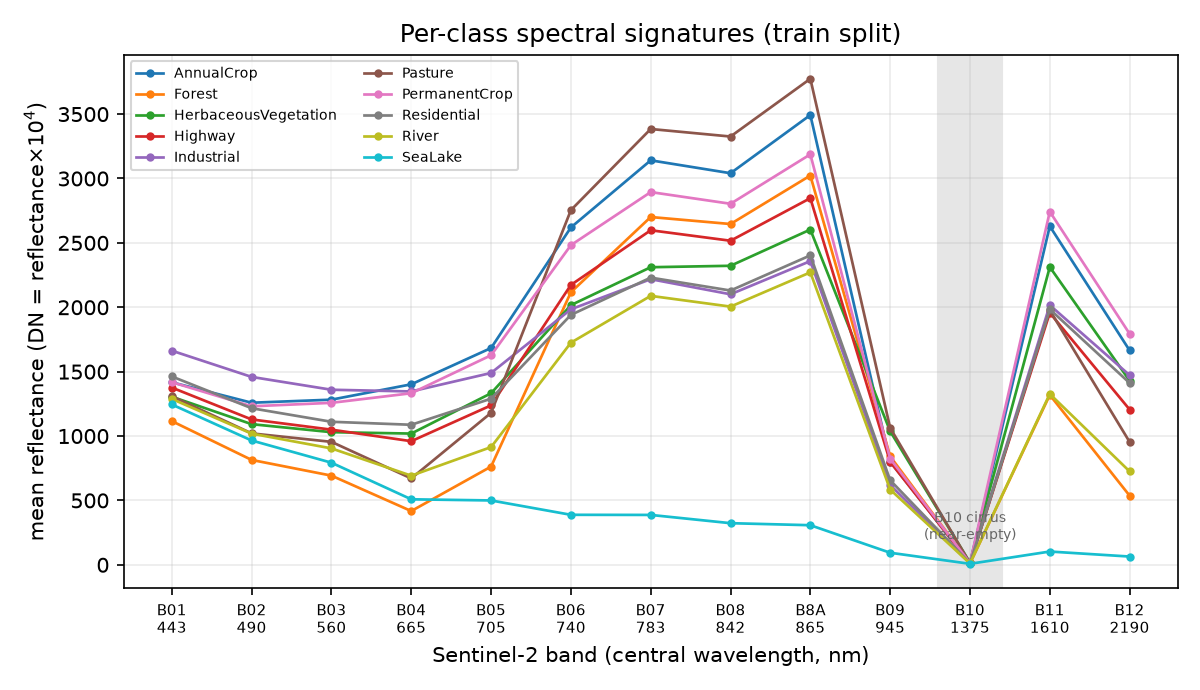
\includegraphics[width=0.78\textwidth]{band_signatures.png}
\caption{Per-class mean spectral signatures. Classes separate most in NIR/SWIR,
not RGB; the highlighted cirrus band B10 is near-empty, justifying its removal.}
\label{fig:sig}
\end{figure}

\section{Methods}
The system has two tiers (Fig.~\ref{fig:pipeline}). \textbf{Tier~1 (classical)}
trains a Random Forest on per-band and per-index summary statistics; it is
interpretable and yields permutation importance directly. Arm C1 uses RGB
statistics; C2 uses the 12 bands plus the four indices.

\begin{figure}[ht]
\centering
\resizebox{\textwidth}{!}{%
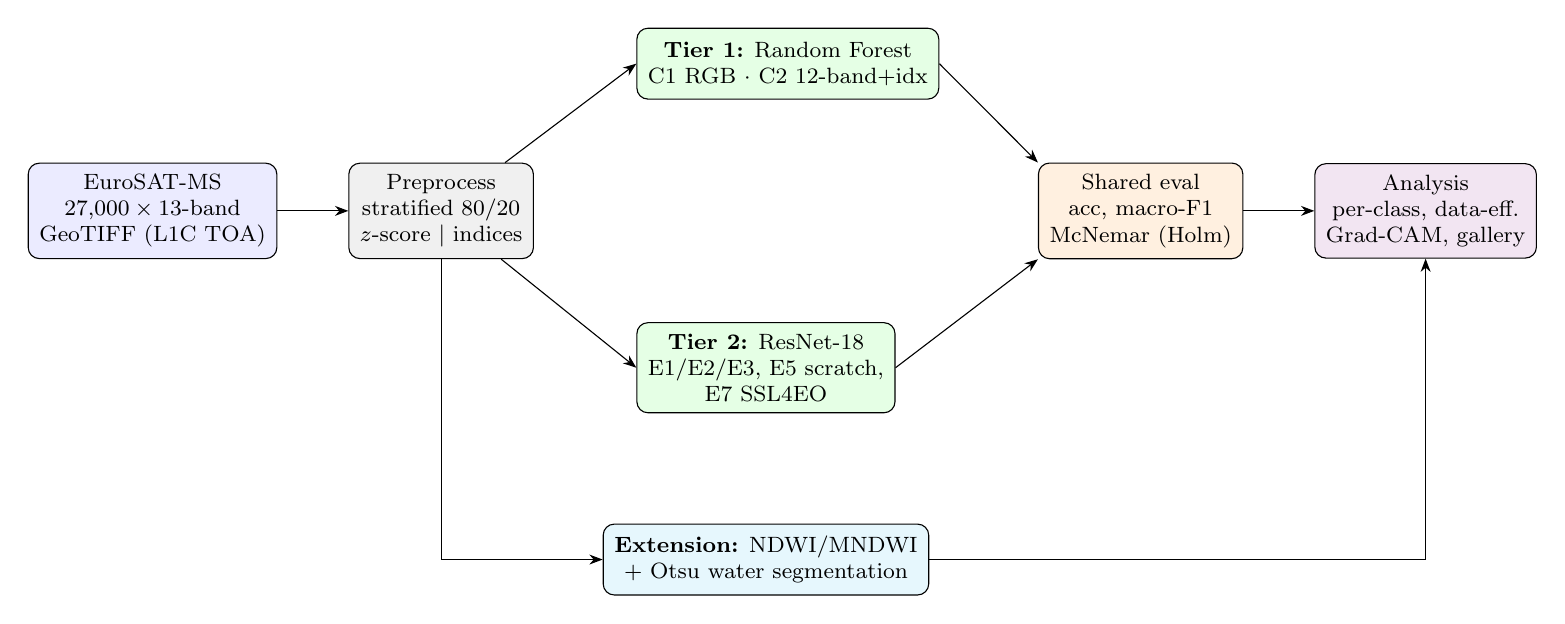
\begin{tikzpicture}[font=\footnotesize, >=Stealth,
  box/.style={draw, rounded corners, align=center, inner sep=4pt, minimum height=9mm},
  data/.style={box, fill=blue!8}, proc/.style={box, fill=black!6},
  tier/.style={box, fill=green!10}, ev/.style={box, fill=orange!12},
  an/.style={box, fill=violet!10}, ext/.style={box, fill=cyan!10}]
\node[data] (d) {EuroSAT-MS\\$27{,}000\times13$-band\\GeoTIFF (L1C TOA)};
\node[proc, right=9mm of d] (p) {Preprocess\\stratified 80/20\\$z$-score $\mid$ indices};
\node[tier, above right=8mm and 13mm of p] (t1) {\textbf{Tier 1:} Random Forest\\C1 RGB $\cdot$ C2 12-band+idx};
\node[tier, below right=8mm and 13mm of p] (t2) {\textbf{Tier 2:} ResNet-18\\E1/E2/E3, E5 scratch,\\E7 SSL4EO};
\node[ev, right=64mm of p] (e) {Shared eval\\acc, macro-F1\\McNemar (Holm)};
\node[an, right=9mm of e] (a) {Analysis\\per-class, data-eff.\\Grad-CAM, gallery};
\node[ext, below=14mm of t2] (seg) {\textbf{Extension:} NDWI/MNDWI\\$+$ Otsu water segmentation};
\draw[->] (d) -- (p);
\draw[->] (p) -- (t1.west);
\draw[->] (p) -- (t2.west);
\draw[->] (t1.east) -- (e.north west);
\draw[->] (t2.east) -- (e.south west);
\draw[->] (e) -- (a);
\draw[->] (p.south) |- (seg.west);
\draw[->] (seg.east) -| (a.south);
\end{tikzpicture}}
\caption{System pipeline. One preprocessing path and one shared evaluator feed
every arm, so the classical and deep tiers are compared on an identical split.}
\label{fig:pipeline}
\end{figure}

\textbf{Tier~2 (deep)} fine-tunes a ResNet-18~\cite{he2016} under one recipe,
selected on the RGB baseline's validation split and applied unchanged to every
arm (AdamW, cosine schedule, $\le 30$ epochs, early stopping on validation
macro-F1), so arms differ only in inputs and pretraining, not tuning. Arm
\textbf{E1} is the ImageNet-pretrained RGB baseline; \textbf{E2} ingests the 12
bands by inflating the first convolution: timm replicates the pretrained RGB
filters across channels and rescales by $3/N$ to preserve activation
magnitude~\cite{carreira2017,wightman2019}. \textbf{E3} appends the four indices
to RGB. To separate \emph{pretraining domain} from \emph{spectral information},
\textbf{E5a/E5b} repeat RGB and 12-band from scratch (no pretraining), and
\textbf{E7/E7b} use SSL4EO-S12 weights (a ResNet-18 self-supervised on
Sentinel-2~\cite{wang2023,stewart2022}) for the 13-band and RGB inputs. E1/E2 and
E7b/E7 together form a $\{$ImageNet, SSL4EO$\}\times\{$RGB, all-band$\}$ design
(Fig.~\ref{fig:design}). As an optional extension I segment water by thresholding
NDWI/MNDWI~\cite{xu2006} with a fixed cut and with Otsu's method~\cite{otsu1979}.

\begin{figure}[ht]
\centering
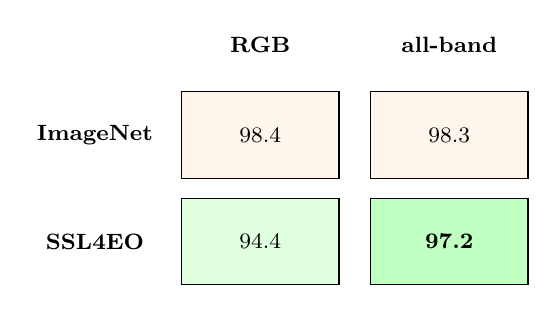
\begin{tikzpicture}[font=\footnotesize,
  c/.style={draw, minimum width=20mm, minimum height=11mm, align=center}]
\node at (0,1.15) {\textbf{RGB}}; \node at (2.4,1.15) {\textbf{all-band}};
\node at (-2.1,0) {\textbf{ImageNet}}; \node at (-2.1,-1.35) {\textbf{SSL4EO}};
\node[c, fill=orange!8] at (0,0) {98.4};
\node[c, fill=orange!8] at (2.4,0) {98.3};
\node[c, fill=green!12] at (0,-1.35) {94.4};
\node[c, fill=green!25] at (2.4,-1.35) {\textbf{97.2}};
\end{tikzpicture}
\caption{Design 2$\times$2 (test accuracy, \%): extra bands help only when
pretraining is in-domain ($+2.8$~pp, bottom row); under ImageNet they tie.}
\label{fig:design}
\end{figure}

\section{Experimental setup}
I follow the mandated 80/20 protocol; the validation slice is used for model
selection and the test set is scored once. The arms whose results carry the
argument (E1, E2, E3 and the E6 data-efficiency sweep at 1/5/10/25\% of the
labels) run at three seeds (reported as mean$\pm$std with per-seed paired
tests); the supporting confound-control and SSL4EO arms run at a single seed
(point estimates) under a fixed compute budget. I report accuracy (mandated)
alongside macro-F1 and per-class recall, given the mild 1.5:1 class imbalance.
Significance uses McNemar's test~\cite{dietterich1998} on the two arms' identical
test predictions, per matched seed; the comparison family is each multispectral
arm versus the RGB baseline, Holm-corrected for multiplicity~\cite{demsar2006}.

\section{Results}
\textbf{Full-data accuracy} (Table~\ref{tab:full}) clusters all deep arms within
0.4~pp at 98.3 to 98.7\%; E3 (RGB+indices) is nominally best at
$98.69\pm0.07$\%. McNemar for E1 versus E2 yields 109 to 151 discordant test
patches and reaches significance in only one of three seeds after correction; at
full data RGB and the 12-band model are statistically indistinguishable, the
expected ceiling effect. E3 edges E1 in one seed.

\begin{table}[ht]
\centering\small
\begin{tabular}{llcc}
\toprule
Arm & Input / pretraining & Accuracy (\%) & Macro-F1 (\%) \\
\midrule
\multicolumn{4}{l}{\emph{Deep, ImageNet-pretrained}}\\
E3 & RGB + indices & $\mathbf{98.69\pm0.07}$ & $98.65$\\
E1 & RGB (baseline) & $98.41\pm0.12$ & $98.36$\\
E2 & 12-band & $98.33\pm0.40$ & $98.27$\\
\multicolumn{4}{l}{\emph{Deep, from scratch / SSL4EO (1 seed)}}\\
E5b & 12-band, scratch & $98.17$ & $98.08$\\
E5a & RGB, scratch & $96.54$ & $96.41$\\
E7 & 13-band, SSL4EO & $97.17$ & $97.05$\\
E7b & RGB, SSL4EO & $94.37$ & $94.25$\\
\multicolumn{4}{l}{\emph{Classical (Random Forest, 1 seed)}}\\
C2 & 12-band + indices & $91.44$ & $91.09$\\
C1 & RGB stats & $79.28$ & $78.47$\\
\bottomrule
\end{tabular}
\caption{Full-data test accuracy (5{,}400-patch test set, identical split).
ImageNet arms tie; spectral information helps under SSL4EO, from scratch, and
classically.}
\label{tab:full}
\end{table}

\textbf{Data efficiency} (Fig.~\ref{fig:de}) tells the opposite of the textbook
hypothesis. With ImageNet pretraining, RGB \emph{beats} multispectral when labels
are scarce: at 1\% of labels ($\sim$190 images) RGB scores
$81.4\pm0.8$\% against $74.7\pm2.5$\% ($-6.7$~pp, and noisier); the gap shrinks
monotonically to $93.3$/$91.9$ at 5\%, $95.7$/$95.3$ at 10\%, and vanishes by
25\% ($96.7$/$96.8$).

\begin{figure}[ht]
\centering
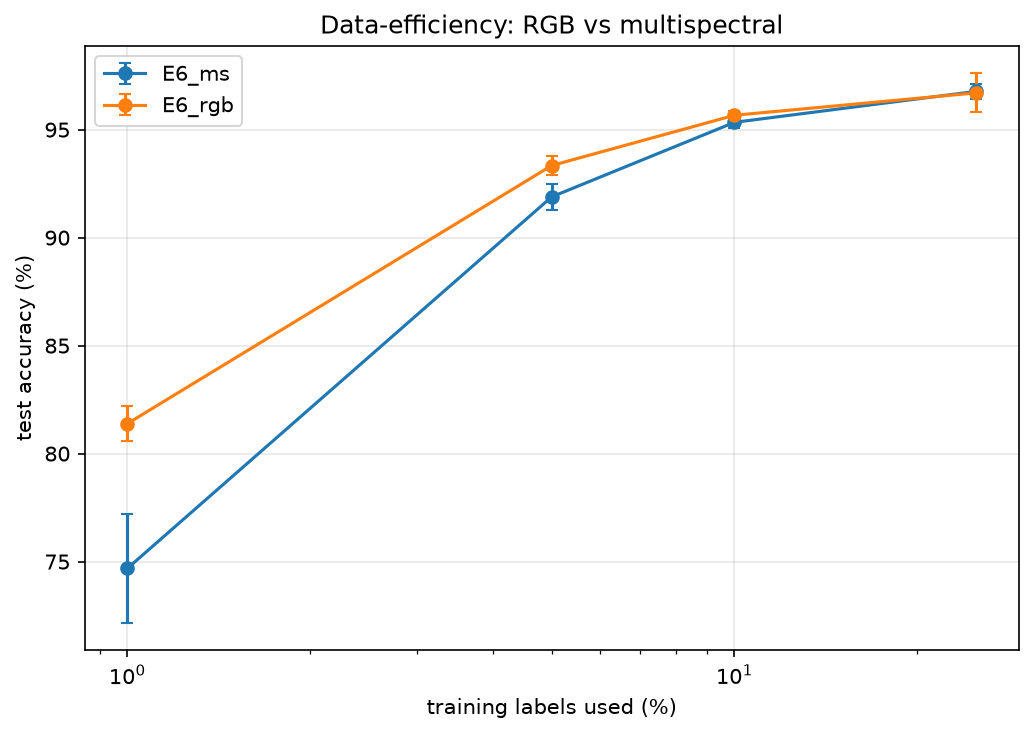
\includegraphics[width=0.64\textwidth]{data_efficiency.png}
\caption{Data-efficiency curve. Under ImageNet pretraining, multispectral trails
RGB most when labels are scarce; the gap closes as data grows.}
\label{fig:de}
\end{figure}

\textbf{Tier-1} reveals the largest spectral effect of the study. Multispectral
features (C2, $91.4$\%) beat RGB features (C1, $79.3$\%) by $+12.2$~pp, with an
overwhelmingly significant McNemar result ($p\approx7\times10^{-106}$, 901
discordant). The per-class gains (Fig.~\ref{fig:tier1}) concentrate exactly where
physics predicts: River $+28$~pp, Highway $+24$, Herbaceous Vegetation $+23$,
Permanent Crop $+20$; the top permutation-importance features are the NDWI and
NDRE indices.

\begin{figure}[ht]
\centering
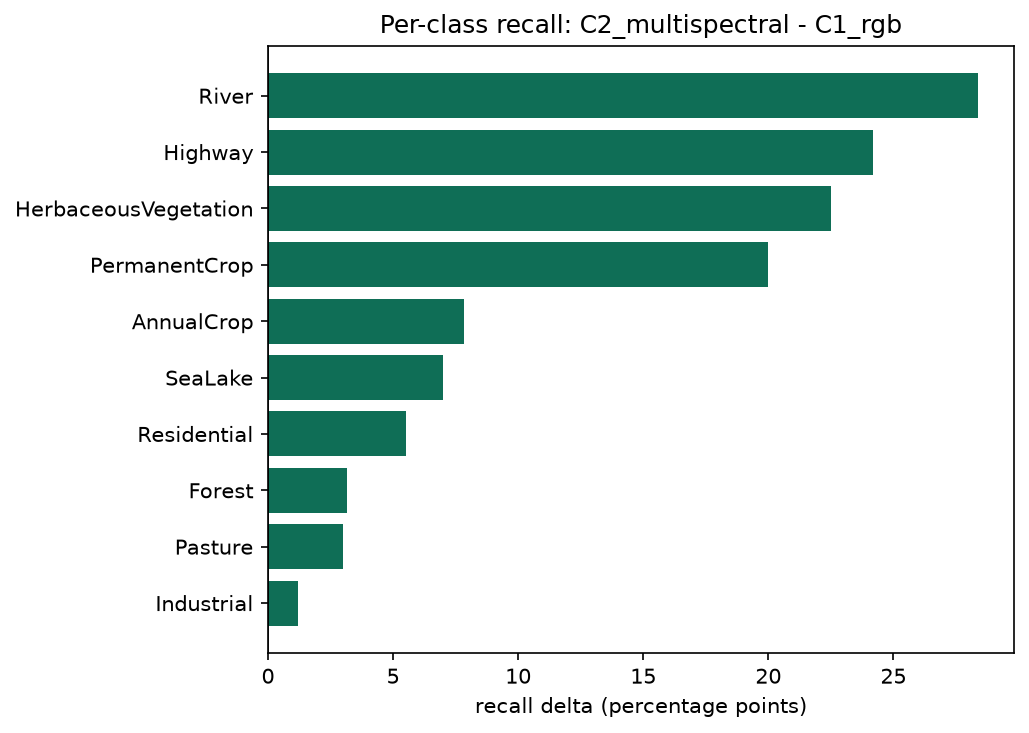
\includegraphics[width=0.6\textwidth]{per_class_delta__C2_multispectral.png}
\caption{Tier-1 per-class recall gain from multispectral features (C2$-$C1).
Gains concentrate on water/impervious and crop-type classes.}
\label{fig:tier1}
\end{figure}

\textbf{The 2$\times$2} (Table~\ref{tab:full}, lower block) points the same way:
under SSL4EO Sentinel-2 pretraining the all-band model beats RGB ($97.2$ vs
$94.4$\%, $+2.8$~pp), the reverse of the ImageNet rows where the two tie.
Training from scratch agrees: 12-band (E5b, $98.2$\%) beats RGB (E5a, $96.5$\%).
These four arms are single-seed point estimates, so I read them as indicative;
the statistical weight rests on the classical and data-efficiency results. The
subjective gallery (Fig.~\ref{fig:gallery}) shows the same classes the confusion
analysis flags (water and crop types) separating cleanly in false-colour and
NDWI views that RGB lacks, and Grad-CAM (Fig.~\ref{fig:gradcam}) shows the RGB and
multispectral models attending to the same discriminative structures (the river
channel, the road junction), so at full data the extra bands add spectral context
rather than redirecting where the network looks.

\begin{figure}[ht]
\centering
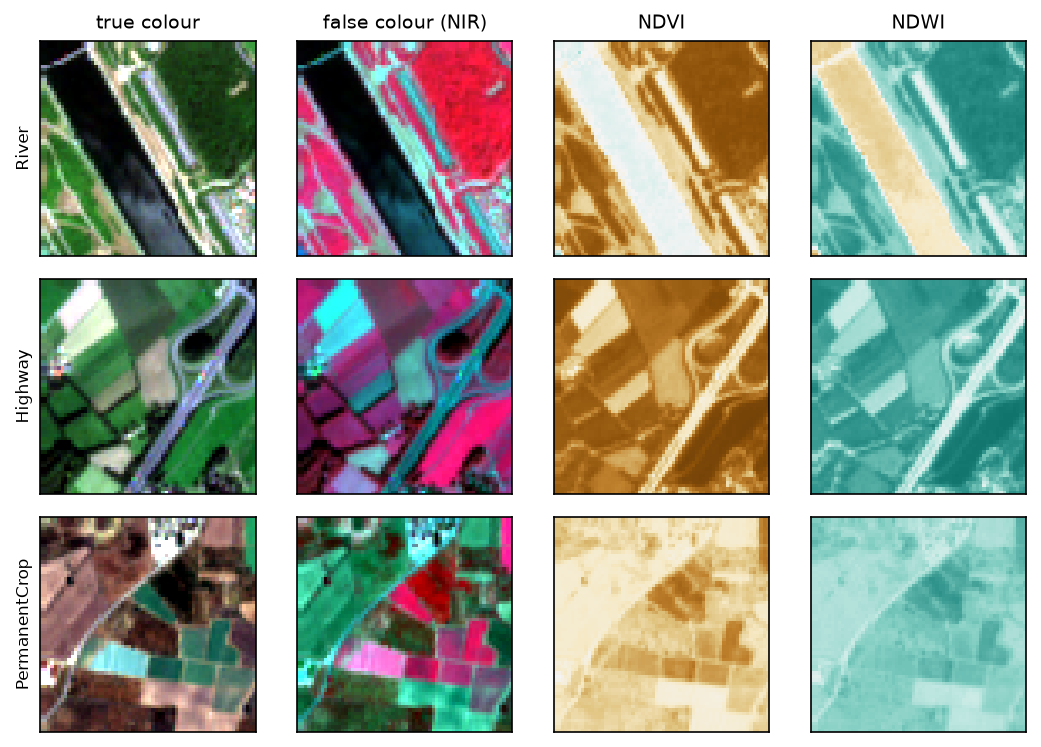
\includegraphics[width=0.6\textwidth]{report_gallery.png}
\caption{Subjective sample, one patch per class: true-colour, false-colour
(NIR), NDVI and NDWI. Water and vegetation separate in the NIR/index views that
RGB cannot see.}
\label{fig:gallery}
\end{figure}

\begin{figure}[ht]
\centering
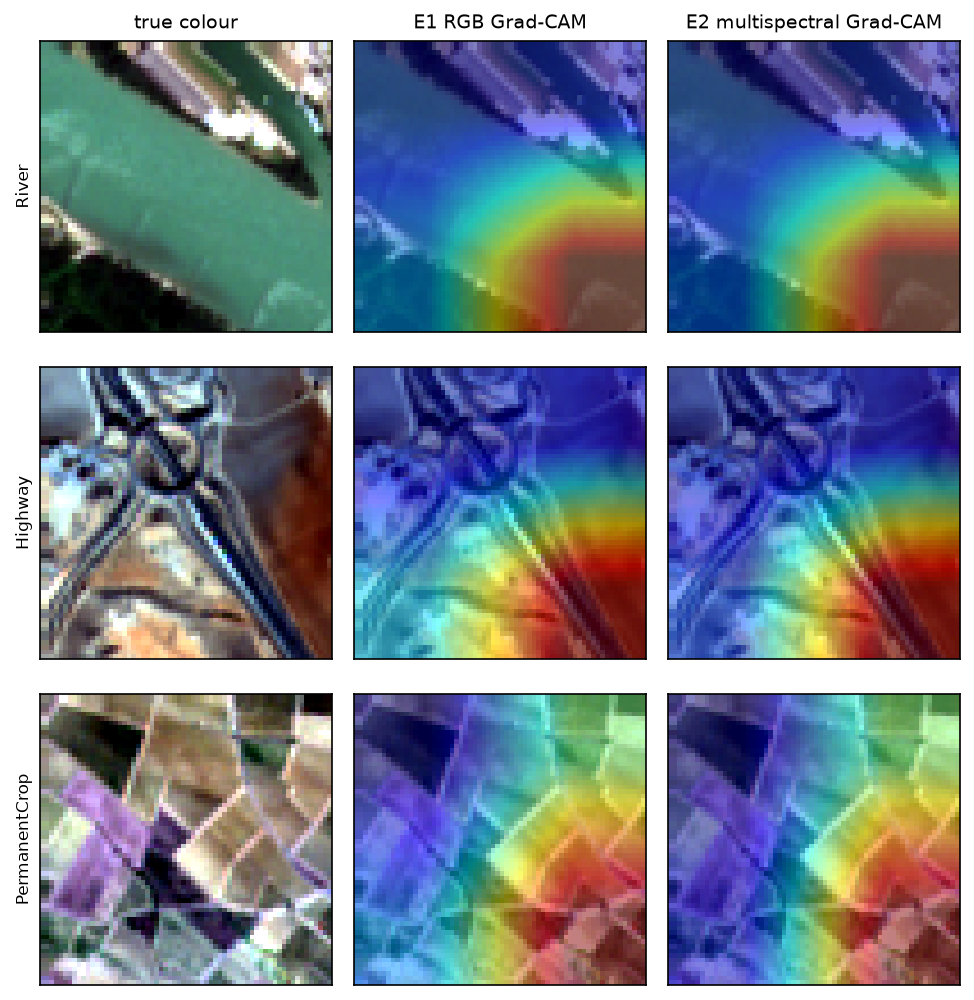
\includegraphics[width=0.6\textwidth]{gradcam.png}
\caption{Grad-CAM for the RGB (E1) and multispectral (E2) models on three test
patches. Both attend to the same discriminative regions, consistent with their
near-identical full-data accuracy.}
\label{fig:gradcam}
\end{figure}

\textbf{Segmentation} (Table~\ref{tab:seg}): on 11 hand-labelled patches,
NDWI+Otsu is best (micro-IoU $0.509$, Dice $0.675$). Otsu beats a fixed
threshold for both indices, and NDWI beats MNDWI, plausibly because the SWIR
bands feeding MNDWI are upsampled from 20~m and blur the thin ($\sim$3~px)
rivers.

\begin{table}[ht]
\centering\small
\begin{tabular}{lcccc}
\toprule
Method & NDWI+fixed & NDWI+Otsu & MNDWI+fixed & MNDWI+Otsu \\
\midrule
micro-IoU  & 0.443 & $\mathbf{0.509}$ & 0.354 & 0.441 \\
micro-Dice & 0.614 & $\mathbf{0.675}$ & 0.523 & 0.612 \\
\bottomrule
\end{tabular}
\caption{Water segmentation on 11 hand-labelled River/Sea-Lake patches.}
\label{tab:seg}
\end{table}

\section{Discussion}
The results resolve ``does multispectral help?'' into ``it depends on the
representation that consumes it.'' Spectral information clearly helps in three
regimes: (i) classical features with no deep pretraining ($+12$~pp); (ii) deep
networks trained from scratch (E5b $>$ E5a); and (iii) deep networks pretrained
in-domain (SSL4EO all-band $>$ RGB). It does \emph{not} help ImageNet-pretrained
networks at full data (where they tie and McNemar is non-significant), and it
actively \emph{hurts} them at low labels, where a 12-channel stem must be adapted
from RGB-shaped filters with too few examples. This reconciles my study with
Helber et al., who reported RGB as their best band combination~\cite{helber2019}:
their networks were ImageNet-pretrained, so their finding is specific to that
regime rather than a property of the data. The Tier-1 per-class gains tie back to
band physics: water and impervious surfaces separate through NIR/SWIR and NDWI,
and crop types through the red edge, which is exactly the information an RGB-only
model cannot see. For an applied multimodal setting, the practical reading is
that additional channels pay off most when the backbone is pretrained in-domain
or trained on the target data, and least when leaning on an RGB-pretrained
representation, particularly under label scarcity.

\section{Limitations and improvements}
The mandated random 80/20 split ignores spatial autocorrelation: EuroSAT patches
cropped from shared Sentinel-2 scenes can leak between train and test, inflating
absolute accuracy~\cite{karasiak2022}. The RGB-versus-multispectral \emph{delta}
shares the split and is partially insulated, but a spatial-holdout robustness
check remains future work. The data are L1C TOA without atmospheric correction,
so indices are discriminative features, not calibrated physical quantities, and
the 20/60~m bands are cubic-spline upsampled, leaving SWIR/red-edge effectively
lower-resolution (visible in the segmentation result). With three seeds, the
reported standard deviations are indicative rather than inferential; my
significance claims rest on McNemar, not on overlapping error bars. The
confound-control and SSL4EO arms are single-seed with no significance test; the
two SSL4EO checkpoints differ in self-supervised pretraining as well as band
count, and the shared recipe was tuned on the RGB baseline (an arm-specific
learning-rate check is future work), so I treat the $2\times2$ and from-scratch
comparisons as indicative. The segmentation evaluation uses only 11 patches with
thin rivers, so its variance is high and it should be read as illustrative.
Natural extensions are a spatial-holdout evaluation, larger or transformer
backbones, L2A surface-reflectance inputs, more seeds, and semi-supervised
methods for the low-label regime~\cite{gomez2021}.

\section{Reproducibility}
The repository contains the full pipeline, committed split manifests,
normalisation statistics, per-seed metrics and all figures.
\texttt{scripts/download\_data.py} fetches the checksum-verified dataset,
\texttt{scripts/make\_manifests.py} regenerates the committed split, and
\texttt{scripts/run\_all.sh} trains every arm and then rebuilds all tables and
figures (analysis, segmentation, Grad-CAM); test suites guard band order, split
integrity and label subsampling.

\FloatBarrier
\begin{thebibliography}{99}\small
\bibitem{helber2019} P.~Helber, B.~Bischke, A.~Dengel, D.~Borth. EuroSAT: A
novel dataset and deep learning benchmark for land use and land cover
classification. \emph{IEEE JSTARS}, 2019.
\bibitem{helber2018} P.~Helber et al. Introducing EuroSAT. \emph{IEEE IGARSS},
2018.
\bibitem{he2016} K.~He, X.~Zhang, S.~Ren, J.~Sun. Deep residual learning for
image recognition. \emph{CVPR}, 2016.
\bibitem{carreira2017} J.~Carreira, A.~Zisserman. Quo vadis, action
recognition? (I3D filter inflation). \emph{CVPR}, 2017.
\bibitem{wightman2019} R.~Wightman. PyTorch Image Models (timm). 2019.
\bibitem{wang2023} Y.~Wang et al. SSL4EO-S12: A large-scale multimodal,
multitemporal dataset for self-supervised learning in Earth observation.
\emph{IEEE GRSM}, 2023.
\bibitem{stewart2022} A.~J.~Stewart et al. TorchGeo: Deep learning with
geospatial data. \emph{ACM SIGSPATIAL}, 2022.
\bibitem{dietterich1998} T.~G.~Dietterich. Approximate statistical tests for
comparing supervised classification learning algorithms. \emph{Neural
Computation}, 1998.
\bibitem{demsar2006} J.~Dem\v{s}ar. Statistical comparisons of classifiers over
multiple data sets. \emph{JMLR}, 2006.
\bibitem{mcfeeters1996} S.~K.~McFeeters. The use of the normalized difference
water index (NDWI). \emph{Int. J. Remote Sensing}, 1996.
\bibitem{xu2006} H.~Xu. Modification of NDWI to enhance open water features
(MNDWI). \emph{Int. J. Remote Sensing}, 2006.
\bibitem{otsu1979} N.~Otsu. A threshold selection method from gray-level
histograms. \emph{IEEE Trans. SMC}, 1979.
\bibitem{karasiak2022} N.~Karasiak et al. Spatial dependence between training
and test sets in remote sensing. \emph{Machine Learning}, 2022.
\bibitem{gomez2021} P.~G\'omez, G.~Meoni. MSMatch: Semi-supervised
multispectral scene classification. \emph{IEEE JSTARS}, 2021.
\end{thebibliography}

\end{document}
